\documentclass{article}
\usepackage[T1]{fontenc}
\usepackage{hyperref, amssymb, amsmath, graphicx}

\setlength{\oddsidemargin}{.25in}
\setlength{\evensidemargin}{.25in}
\setlength{\textwidth}{6in}
\setlength{\topmargin}{-0.4in}
\setlength{\textheight}{8.5in}

\setlength{\parindent}{0in}
\setlength{\parskip}{8pt}

\newcommand{\heading}[6]{
	\renewcommand{\thepage}{#1-\arabic{page}}
	\noindent
	\begin{center}
	\framebox{
		\vbox{
			\hbox to 5.78in { \textbf{#2} \hfill #3 }
			\vspace{4mm}
			\hbox to 5.78in { {\Large \hfill #6  \hfill} }
			\vspace{2mm}
			\hbox to 5.78in { \textit{Instructor: #4 \hfill #5} }
		}
	}
	\end{center}
	\vspace*{4mm}
}

\newtheorem{theorem}{Theorem}
\newtheorem{definition}[theorem]{Definition}
\newtheorem{remark}[theorem]{Remark}
\newtheorem{lemma}[theorem]{Lemma}
\newtheorem{corollary}[theorem]{Corollary}
\newtheorem{proposition}[theorem]{Proposition}
\newtheorem{claim}[theorem]{Claim}
\newtheorem{observation}[theorem]{Observation}
\newtheorem{fact}[theorem]{Fact}
\newtheorem{assumption}[theorem]{Assumption}

\newenvironment{proof}{\noindent{\bf Proof:} \hspace*{1mm}}{
	\hspace*{\fill} $\Box$ }
\newenvironment{proof_of}[1]{\noindent {\bf Proof of #1:}
	\hspace*{1mm}}{\hspace*{\fill} $\Box$ }
\newenvironment{proof_claim}{\begin{quotation} \noindent}{
	\hspace*{\fill} $\diamond$ \end{quotation}}
	
\newcommand{\lecture}[4]{\heading{#1}{ECE4880J: Computer Vision}{#2}{Siheng Chen}{#4}{#3}}



%%%%%%%%%%%%%%%%%%%%%%%%%%%%%%%%%%%%%%%%%%%%%%%%%%%%%%%%%%%%%%%%%%%%%%%%%%%%%%%
% PLEASE MODIFY THESE FIELDS AS APPROPRIATE:
\newcommand{\lecturenum}{X} % lecture number
\newcommand{\lecturedate}{May 15, 2022} % date of lecture (e.g., 'March 20, 2010')
\newcommand{\lecturetitle}{Homework 2: Python Programming} % lecture title
\newcommand{\scribename}{{\bf Yiwen Yang}} % full name of scribe
% PUT HERE ANY PACKAGES, MACROS, etc., ADDED BY YOU
%
%%%%%%%%%%%%%%%%%%%%%%%%%%%%%%%%%%%%%%%%%%%%%%%%%%%%%%%%%%%%%%%%%%%%%%%%%%%%%%%
\usepackage{hyperref}
\usepackage[section]{placeins}
\usepackage{caption}
\usepackage{subcaption}

%%%%%%%%%%%%%%%%%%%%%%%%%%%%%%%%%%%%%%%%%%%%%%%%%%%%%%%%%%%%%%%%%%%%%%%%%%%%%%%
\begin{document}
\lecture{\lecturenum}{\lecturedate}{\lecturetitle}{\scribename}


\section*{Instruction}

\begin{itemize}
		\item This homework is due at 11:59:59 p.m. on ** May 30th, 2022.
		\item The write-up must be an electronic version edited by LATEX using \textbf{this template} and submitted in \textbf{pdf} format.
		\item Please DO NOT rename python files and their functions. Just fill it. 
		\item The overall submission should be a .zip file named by xxx(student id)-xxx(name)-Assignment2.zip
\end{itemize}


{\bf Python Environment.} We are using \href{https://docs.python.org/3.7/library/index.html}{Python 3.7} for this course. We will use the following packages in this course:
\href{https://numpy.org/}{Numpy},
\href{https://scipy.org/}{SciPy},
\href{http://matplotlib.org/users/pyplot tutorial.html}{Matplotlib},
\href{https://pytorch.org/}{Pytorch}.

\section*{Q2. Numpy}

\begin{figure}[!hbtp]
	\centering
	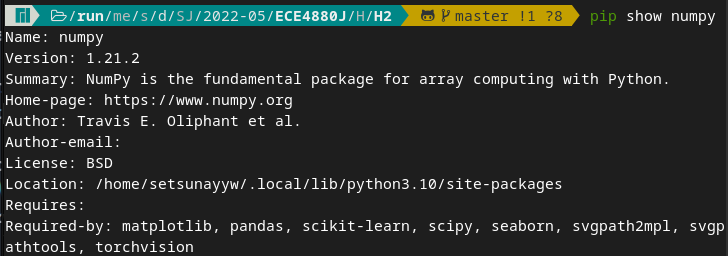
\includegraphics[width=0.8\textwidth]{img/np-version.png}
	\caption{\label{fig:np-version}Numpy Version}
\end{figure}

\section*{Q3. SciPy}

\begin{figure}[!hbtp]
	\centering
	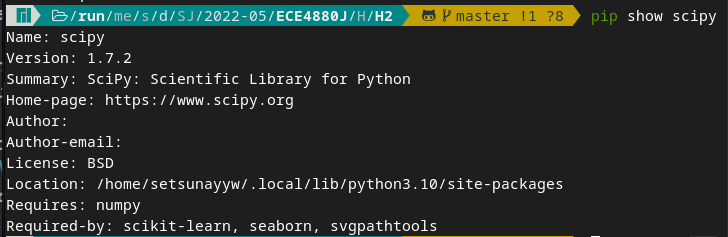
\includegraphics[width=0.8\textwidth]{img/scipy-version.png}
	\caption{\label{fig:scipy-version}SciPy Version}
\end{figure}

\section*{Q4. Matplotlib}

\begin{figure}[!hbtp]
	\centering
	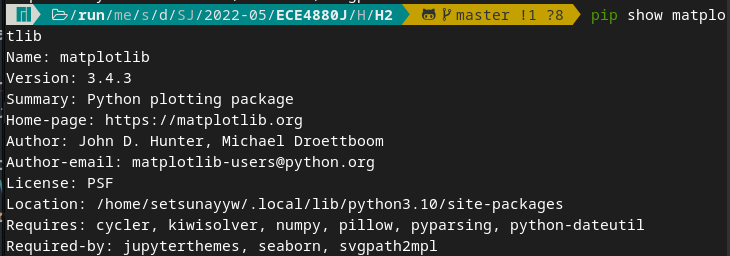
\includegraphics[width=0.8\textwidth]{img/matpl-version.png}
	\caption{\label{fig:matpl-version}Matpltlib Version}
\end{figure}

\section*{Q5. Pytorch}

\begin{figure}[!hbtp]
	\centering
	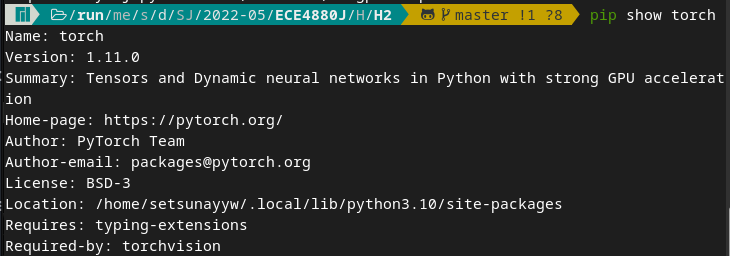
\includegraphics[width=0.8\textwidth]{img/torch-version.png}
	\caption{\label{fig:torch-version}PyTorch Version}
\end{figure}

\begin{figure}
	\centering
	\begin{subfigure}[b]{0.4\textwidth}
		\centering
		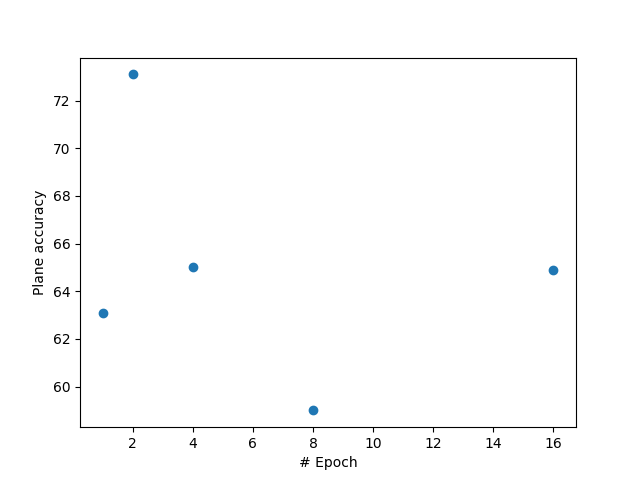
\includegraphics[width=\textwidth]{img/epoch_accuracy.png}
		\caption{\label{fig:epoch-acc}Accuracy of plane classification vs. traning epoch}
	\end{subfigure}
	\hfill
	\begin{subfigure}[b]{0.4\textwidth}
		\centering
		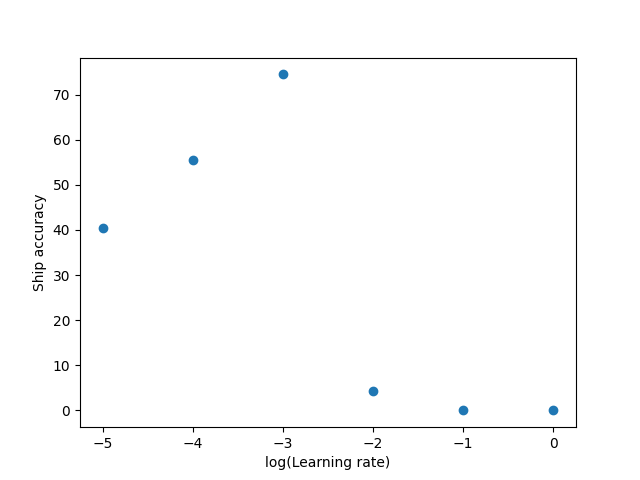
\includegraphics[width=\textwidth]{img/lr_accuracy.png}
		\caption{\label{fig:lr-acc}Accuracy of ship classification vs. learning rate}
	\end{subfigure}
	\caption{\label{fig:acc}Accuracy Test}
\end{figure}

The accuracy of "plane" classification with a fixed learning rate $lr=10^{-3}$ changes according to the training epoch, as shown in Figure \ref{fig:epoch-acc}. The best epoch is estimated to be 2, with accuracy $73.1\%$.

The accuracy of "ship" classification with a fixed training epoch as 4 changes according to the learning rate, as shown in Figure \ref{fig:lr-acc}. The best learning rate is estimated to be $10^{-3}$, with accuracy $74.5\%$.

When changing the loss function from crossentropy to MSE and set learning rate at $10^{-3}$ with epoch of $2$, the accuracy of "plane" classification is $66.6\%$ and "ship" is $58.4\%$. The accuracy is lower comparing to crossentropy, but if epoch is set $4$, the accuracy of "plane" is highest at $71.0\%$ and "ship" is $68.4\%$, inferring that with MSE as the loss function one may have loop more to achieve higher accuracy.


% bibliography goes here
\bibliographystyle{amsalpha}

\end{document}
%%%%%%%%%%%%%%%%%%%%%%%%%%%%%%%%%%%%%%%%%%%%%%%%%%%%%%%%%%%%%%%%%%%%%%%%%%%%%%%